%%%%%%%%%%%%%%%%%%%%%%%%%%%%%%%%%%%%%%%%%%%%
\chapter{Experimental Design}
%%%%%%%%%%%%%%%%%%%%%%%%%%%%%%%%%%%%%%%%%%%%
\begin{center}
  \begin{minipage}{0.75\textwidth}
    \begin{small}
      ““I have not failed. I've just found 10,000 ways that won't work”.\\
      \null\hfill\emph{Thomas Edison}
    \end{small}
  \end{minipage}
  \vspace{0.5cm}
\end{center}

In order to demonstrate the effectiveness of polarization and texture features with support vector machines for the purpose of classification and relative water content determination, experiments were designed, conducted and analyzed. These experiments was designed to investigate the linear polarizance vector of the Mueller matrix for various species of tree leaves in the diffuse and specular directions.  Leaves were investigated in different physiological states determined by both decomposition time and relative water content.  Classification and regression techniques were used to correlate the polarization and texture information from images acquired of various species of leaves.  Data for Red Oak, American Ash and Sugar Maple leaves was acquired for the purpose of classification.  Devils Ivy was observed in studies on relative water content.

Specular reflections are well known to create highly polarized light \cite{grant},\cite{vanderbilt}. The diffuse portion of reflection has been less investigated.  It has often been assumed that the diffuse portion is unpolarized due to multiple scattering and volume scattering caused by type B and C photons creating random orientations of light.  Recently the polarization of the diffuse component has been observed in studies \cite{surface}, \cite{shapediffuse} for the purpose of determining the geometry of various surfaces.  In the experiments on individual plant leaves reported here the diffuse portion was observed for indicators of physiological, chemical, and biological status. It was assumed that as the leaf surfaces decompose or lose water content, the surface would become rougher as the epicuticle wax layer changed. The experiments presented here, attempt to demonstrate results that agree with previously outlined light leaf interactions in the specular direction, as well as extend the analysis to the diffuse direction.  The acquired polarization and texture data was processed for the purpose of determining the surface texture and internal scattering mechanisms for classification between various species and investigation into the differences in these processes during decomposition and water stress conditions.

There are numerous challenges to the practical application of BRDF models due to the large amount of measurements required to classify an object's reflective polarization properties.  A digital microscope was utilized for the purpose of quantifying regions on leaves that include different surface structures such as veins, mold, undulations, cell walls, etc.

The polarizance of a material represents the first column of its Mueller Matrix, and determines the amount of polarization that results from unpolarized incident light.  These elements represent the linear polarization that results from the light material interactions and can be useful for characterizing a material.  The polarizance can easily be acquired using simple light measuring Polarimetry techniques when the incident light is unpolarized.  The measurements required to determine this vector is severely reduced when compared to other measurement techniques.

All measurements were performed using light incident at approximately the Brewster angle of 55 degrees. This is the Brewster angle calculated between air $n=1.0$ and glass $n=1.5$.  The index of refraction for leaves is estimated to be between 1.3 and 1.6. Specular observations were observed at 55 degrees from the normal to the plane of incidence.  The diffuse measurements were taken at 0 degrees from the normal.

The Brewster angle was chosen since it represents the angle where light reflected from an ideal specular surface would be highly polarized.  In the natural environment, leaves are in various orientations to the normal surface of a plant canopy.  It is typical to extend the results from micro level leaf studies to canopies by creating probability distribution models that can predict the various leaf orientations.  Combining the results from individual leaf studies with probability models should provide more accurate information for interpreting plant image data. The experimental setups for the specular and diffuse components can be found in  Figure 3.1 and Figure 3.2.
%
\begin{figure}[!htb]
    \begin{center}
        \makebox[\textwidth]{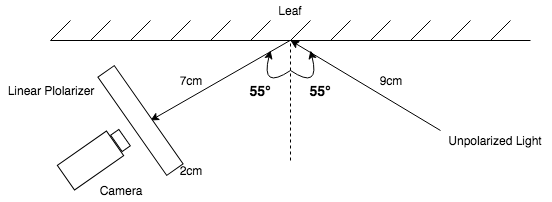
\includegraphics[scale=0.5]{/Sources/Experimental_Design/specular-exp.png}}
    \end{center}
    \caption{Specular Experimental Setup}
    \label{fig:Experiment}
\end{figure}
\begin{figure}[!htb]
    \begin{center}
        \makebox[\textwidth]{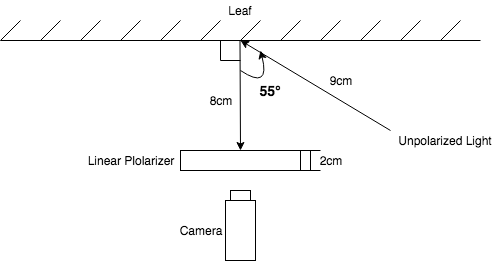
\includegraphics[scale=0.5]{/Sources/Experimental_Design/diffuse-experiment.png}}
    \end{center}
    \caption{Diffuse Experimental Setup}
    \label{fig:Experiment}
\end{figure}
%
Using measurements acquired through a linear polarizer, the polarizance of each sample was calculated and plotted as a histogram.  The measurements were acquired using a digital microscope which produced images for each orientation of the polarizing filter.  These images were additionally processed for texture feature extraction using GLCM techniques.
%TODO: provide noise analysis of images using x,y,z techniques
Each color image was split into individual color channels in order to apply greyscale imaging techniques. This is known as pseudo-spectral analysis, or PSA.

Extracted features were observed and utilized for the purpose of classification among species and determining the relative water content of individual leaves using regression analysis.  For each type of experiment, the same orientation of polarizer and camera was used to capture images in the diffuse and specular directions.
